% Auteur\,: Steve Prud’Homme
% Cette oeuvre, création, site ou texte est sous licence Creative Commons Attribution - Pas d’Utilisation Commerciale - Partage dans les Mêmes Conditions 4.0 International. Pour accéder à une copie de cette licence, merci de vous rendre à l'adresse suivante 
% http://creativecommons.org/licenses/by-nc-sa/4.0/ ou envoyez un courrier à 
% Creative Commons, 444 Castro Street, Suite 900, Mountain View, California, 94041, USA.

%\,:::SNIPET
%\,::: SECTION
% \section{Contexte} 
%		\begin{frame}[allowframebreaks]
%			\frametitle{}
%			\begin {itemize}
%				\item 
%			\end{itemize}
%		\end{frame}
%:::WATER MARK / FILIGRANE
%\usepackage{draftwatermark}
%\SetWatermarkLightness{0.5}
%\SetWatermarkAngle{25}
%\SetWatermarkScale{0.5}
%\SetWatermarkFontSize{2cm}
%\SetWatermarkText{Document de travail}


\documentclass{beamer}
\usepackage{color}
\usepackage{beamerthemesplit} % new 
\usepackage[french]{babel}
\usepackage[utf8]{inputenc}
\usepackage{tikz}
\usepackage[fixlanguage]{babelbib}
\selectbiblanguage{french}
% Natlib pour la bibliographie
\usepackage{natbib}
\usepackage{url}
\usetikzlibrary{mindmap,shadows,shapes,backgrounds}
\usepackage[T1]{fontenc}
\setbeamertemplate{bibliography item}[text]
\usepackage{multicol}


\definecolor{MightySlate}{RGB}{85,98,112}
\definecolor{Pacifica}{RGB}{78,205,196}
\definecolor{AppleChic}{RGB}{199,244,100}
\definecolor{CheeryPink}{RGB}{255,107,107}

\setbeamercolor{titlelike}{parent=structure}
\setbeamerfont*{title}{size=\huge}
\setbeamercolor{title}{bg=MightySlate, fg=white}
\setbeamercolor{author}{bg=Pacifica, fg=white}
\setbeamercolor{institute}{bg=AppleChic, fg=black}
\setbeamercolor{date}{bg=CheeryPink, fg=white}

\definecolor{DTUred}{RGB}{178,20,20}
\setbeamercolor*{palette primary}{use=structure,fg=white,bg=MightySlate}
\usepackage{helvet}
%\usepackage{draftwatermark}
%\SetWatermarkLightness{0.5}
%\SetWatermarkAngle{25}
%\SetWatermarkScale{0.5}
%\SetWatermarkFontSize{2cm}
%\SetWatermarkText{Document de travail}

\begin{document}
	\title{Plan d’action de conception et réalisation de projets de formation en ligne} 
	\subtitle{Évaluation}
	\author{Steve Prud'Homme} 
	\institute{Commission scolaire de Laval} 
	\date{\today} 

	
	%\usebackgroundtemplate{%
  %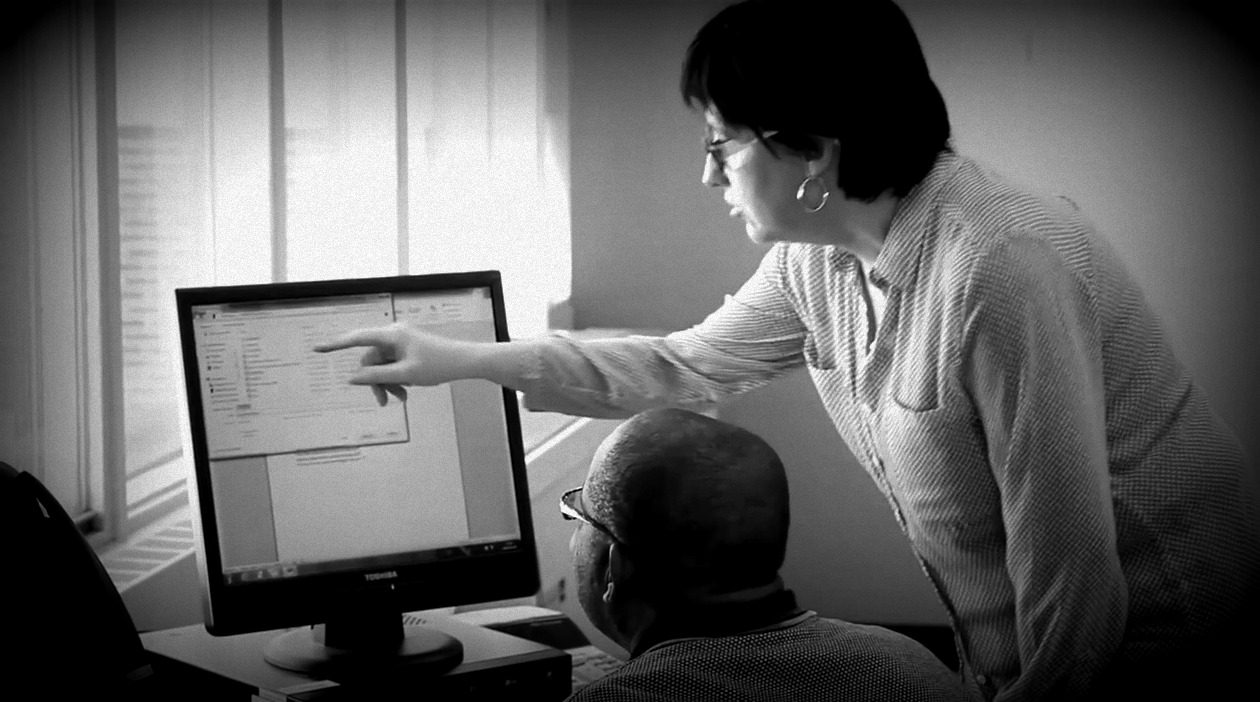
\includegraphics[height=\paperheight]{back.png}} 
	
	\frame{\titlepage} 
    
	\usebackgroundtemplate{ } 
	\par L’intention de ce document est de respecter pleinement les droits des créateurs des ressources
utilisées.
	\par En ce qui concerne les citations insérées selon le principe de l'utilisation équitable ou avec la permission de l'auteur, veuillez les contacter ou respecter les droits d’utilisation précisés dans les documents d’origine avant de les réutiliser.
	\par Si vous estimez que certains éléments de ce rapport ne respectent pas intégralement les droits de vos
publications, veuillez nous en aviser afin que les modifications nécessaires puissent être apportées au\,: \url{mailto:sprudhomme@cslaval.qc.ca}.
	\par Cette \oe uvre, création, site ou texte est sous licence Creative Commons Attribution\,-\,Pas d’Utilisation Commerciale\,-\,Partage dans les Mêmes Conditions 4.0 International.	\section{Sommaire} 
		\begin{frame}
			Cette présentation vise à\,:
			\frametitle{Sommaire}
			\begin {itemize}
				\item \textbf{Familiariser} l'auditoire sur les des situations de travail, les processus de production, 
du contrôle de la qualité et  les  bonnes pratiques en conception et réalisation d’outils pédagogiques en ligne en présentant un bref aperçu de la \textbf{littérature} et de notre survol.
				\item Démontrer qu'il est pertinent d'adopter des \textbf{pratiques harmonisées}.
				\item Promouvoir l'idée qu'il serait pertinent de \textbf{concevoir une norme, accréditation ou un cadre de référence en ce qui concerne conception et réalisation d’outils pédagogiques en ligne}.

			\end{itemize}
		\end{frame}
	\frame[allowframebreaks]{\frametitle{Ordre du jour}\tableofcontents}


	\section{Introduction} 
		
		
	\subsection{Présentateur} 
		\begin{frame}[allowframebreaks]
			\begin {itemize}
				      \item 
			\end{itemize}
		\end{frame}           
						
						
%\section{Bibliographie}
%\subsection{Bibliographie}
\frame[allowframebreaks]{\frametitle{Bibliographie}

\bibliographystyle{apalike}
\bibliography{bibliographie} %bibtex file name without .bib extension
}
\framebreak
\par L’intention de ce document est de respecter pleinement les droits des créateurs des ressources
utilisées.
	\par En ce qui concerne les citations insérées selon le principe de l'utilisation équitable, veuillez les contacter ou respecter les droits d’utilisation précisés dans les documents d’origine avant de les réutiliser.
	\par Si vous estimez que certains éléments de ce rapport ne respectent pas intégralement les droits de vos
publications, veuillez nous en aviser afin que les modifications nécessaires puissent être apportées au\,: \url{mailto:sprudhomme@cslaval.qc.ca}.
	\par Cette \oe uvre, création, site ou texte est sous licence Creative Commons Attribution\,-\,Pas d’Utilisation Commerciale\,-\,Partage dans les Mêmes Conditions 4.0 International. \\
	\par 
	 Pour accéder à une copie de cette licence, merci de vous rendre à l'adresse suivante\,: \url{http://creativecommons.org/licenses/by-nc-sa/4.0/} ou envoyez un courrier à 

\par Creative Commons, 444 Castro Street, Suite 900, Mountain View, California, 94041, USA.
\par Ce document a été réalisé en \LaTeX, avec l'environnement Beamer. Vous pouvez trouver le code source ici\,: \url{https://goo.gl/43zjqQ}. Vous pouvez avoir accès à cette présentation ainsi qu'à d'autres ressources sur\url {https://goo.gl/wqpUh6}
\end{document}

